% +------------------------------------------------------------------------+
% | CGAL Reference Manual:  Subdivision_surfaces_3
% +------------------------------------------------------------------------+
% | Subdivision surfaces on generic Polyhedron.
% | 
% | 1.2.2005  Le-Jeng Andy Shiue
% |
\RCSdef{\subdivisionRev}{$Revision$}
\RCSdefDate{\subdivisionDate}{$Date$}
% +------------------------------------------------------------------------+

\newcommand\DS{Doo-Sabin}

% ------------------------------------------------------------------------
\newcommand\FIGDIR{Subdivision_surfaces_3/FIG}
\newcommand\IL{{\itshape left}}
\newcommand\IR{{\itshape right}}
\newcommand\IM{{\itshape middle}}
\newcommand\IT{{\itshape top}}
\newcommand\IB{{\itshape bottom}}
% ------------------------------------------------------------------------

\ccParDims

\chapter{Subdivision Surfaces}
\label{chapterSubdivision}
\ccChapterRelease{\subdivisionRev. \ \subdivisionDate}
\ccChapterAuthor{Le-Jeng Andy Shiue}
\hspace{.4cm}
\begin{ccTexOnly}
    \setlength{\unitlength}{1mm}
    \begin{picture}(0,0)(0.0,0.0)
      \put (78,25){% textwidth = 156mm
          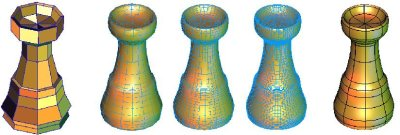
\includegraphics[width=0.45\textwidth]{\FIGDIR/QTSub}
      }
    \end{picture}\vspace{-4mm}% compensate for some vspace added by picture
\end{ccTexOnly}

\minitoc

% +------------------------------------------------------------------------+
\section{Introduction} \label{sectionSubIntro}
% +------------------------------------------------------------------------+
The subdivision algoithm is an easy to use yet powerful way to generate smooth 
surfaces from simple polyhedron meshes. Unlike spline-based surfaces
(e.g NURBS) or other numeric-based modeling techniques, users of subdivision
surfaces are not required to have in-depth mathematics knowledge on subdivision 
algorithms. An artist just need some natural geometric intuitions 
to control the subdivision surfaces. It is hence especilally 
popular for the character modeling in video games and character animations.

%Subdivision algorithms (see e.g.~\cite{cgal:ww-smgd-02})
%recursively refine coarse meshes and generate ever closer 
%approximations to a smooth surface.
%for character animation, surface modeling, or physics simulation.
%Setting aside the specific strategy of geometric averaging
%for the new points, subdivision algorithms can be classified 
%according to the topological refinement of the underlying mesh.
%\ccc{Subdivision_surfaces_3}, working on the concept of the 
%\ccc{CGAL::Polyhedron_3} (see Chapter~\ref{chapterPolyhedron}),
%takes advantage of this separation of geometry and topology.
%Each subdivision algorithm is a refinement function parametrized
%by a set of rountines of geometric averageing.

While many subdivision schemes are developed and new schemes are 
still being researched, \ccc{Subdivision_surfaces_3} supports the families 
of the four most used schemes: Loop, Catmull-Clark,
Doo-Sabin and $\sqrt{3}$ subdivisions. \ccc{Subdivision_surfaces_3}, 
working on the concept of the \ccc{CGAL::Polyhedron_3} (see 
Chapter~\ref{chapterPolyhedron}), aims to be easy to use and powerful to
extend.

\begin{ccHtmlOnly}
     <CENTER>
         <img src="./FIG/QTSub.jpg" alt="QT subdivision on a rook model"><P>
     </CENTER>
\end{ccHtmlOnly}

% +------------------------------------------------------------------------+
\section{Subdivision Algorithms}
% +------------------------------------------------------------------------+
In this chapter, we try to explain some fundamentals of subdivision 
surfaces. We only focus on the topics helping you to understand the 
design of the package; for interested readers, \cite{cgal:ww-smgd-02} 
gives an in-depth introduction.
You can fast-forward to the next section if you 
just want to apply Loop (or Catmull-Clark ...etc) subdivision on your
\ccc{CGAL::Polyhedron_3} mesh.

Subdivision algorithms recursively refine coarse meshes and generate 
ever closer approximations to a smooth surface.
%Subdivision algorithms (see e.g.~\cite{cgal:ww-smgd-02}) 
%define surfaces as the limit
%of recursive refinement of a polyhedral mesh, called
%\emph{control mesh}. 
%The refinements generate mesh points 
%to be smoothed to approximate the limit surface.   
The chapter teaser shows a sequence of a subdivision on 
a chess model. The input mesh is called 
\emph{control mesh}.

Four popular refinment patterns are used in practice, and each of them
is used by Loop, Catmull-Clark\cite{cgal:cc-rgbss-78}, Doo-Sabin 
and $\sqrt{3}$ subdivision.

\begin{ccTexOnly}
  \begin{center}
    \parbox{0.6\textwidth}{%
      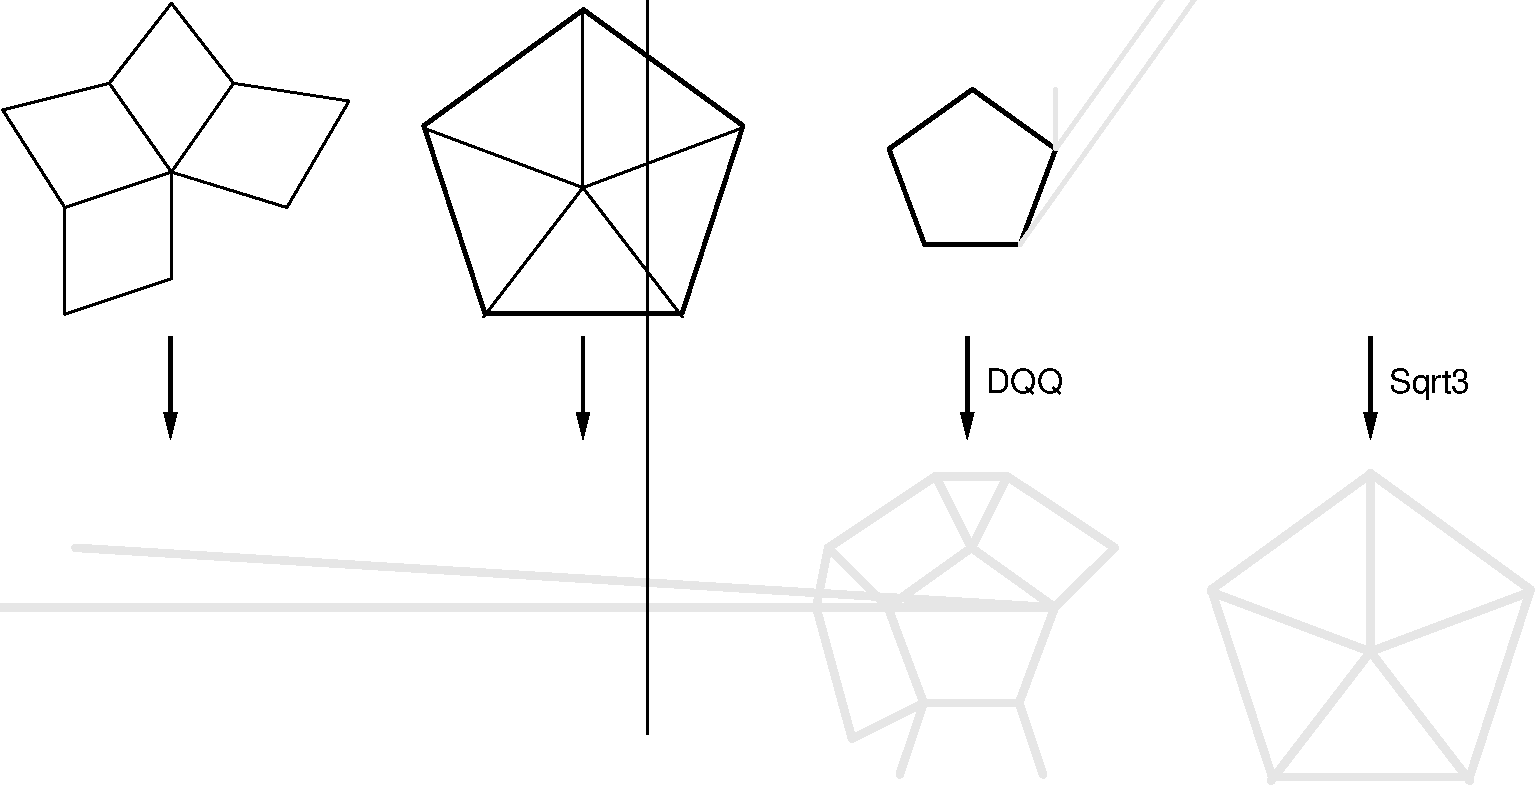
\includegraphics[width=0.6\textwidth]{\FIGDIR/RefSchemes}%
    }\\ \vspace{0.5cm}
    The refined mesh is shown below the control mesh.
  \end{center}
\end{ccTexOnly}

\begin{ccHtmlOnly}
  <CENTER>
     <img src="./FIG/RefSchemes.gif" alt="Refinement Hosts"></A><P>
  </CENTER>
\end{ccHtmlOnly}

Points on the refined mesh are generated by averaging
neighbor points on the input mesh. A graph, called \emph{stencil}, 
determines the input submesh whose points contribute to the 
position of a refined point. 
%Stencils are defined at the time the refinement pattern is chosen.  
%as illustrated in Figure \ref{fig:RefMap},
For example, the 
%\emph{P}rimal \emph{Q}uadtrateral \emph{Q}uadrisection (PQQ) scheme 
refinement used by Catmull-Clark subdivision has a vertex-node stencil, 
which defines the 1-ring of an input vertex; an edge-node stencil, 
which defines the 1-ring of a input edge; and a facet-node stencil, 
which defines an input facet.

\begin{ccTexOnly}
  \begin{center}
    \parbox{0.5\textwidth}{%
      
\includegraphics[width=0.5\textwidth]{\FIGDIR/PQQStencil}%
    }\\ \vspace{0.5cm}
    The blue neighborhoods in the top row indicate the corresponding
    stencils of the refined nodes in red. 
  \end{center}
\end{ccTexOnly}

%while the DQQ scheme has only a corner-node stencil, which 
%relates the facet of a corner to a target node.
Stencils with weights are called \emph{geometry masks}.
%One practical set of geometry masks of the PQQ scheme is
The geometric masks of Catmull-Clark subdivision are shown below.

\begin{ccTexOnly}
  \begin{center}
    \parbox{0.4\textwidth}{%
      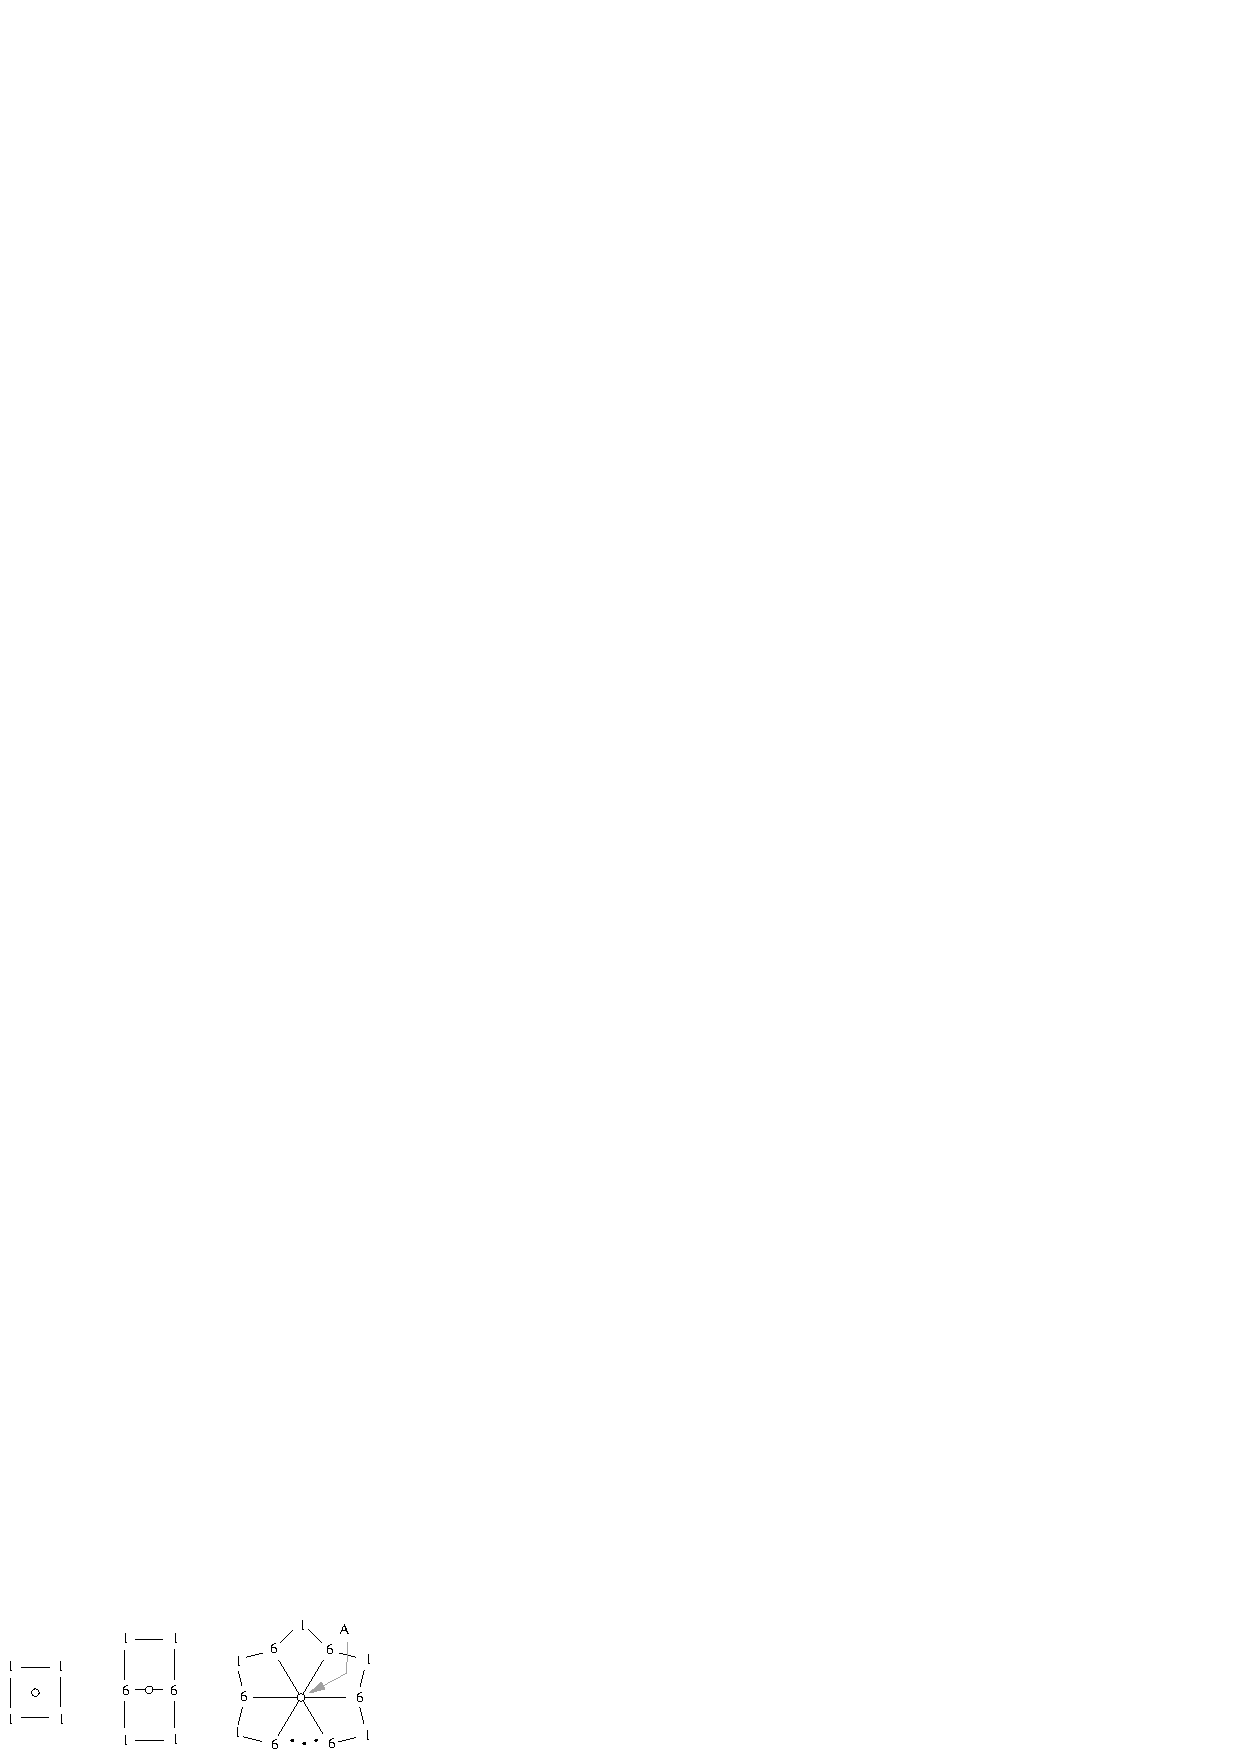
\includegraphics[width=0.4\textwidth]{\FIGDIR/cc_mask}%
    } \\ \vspace{0.5cm}
    The red nodes indicates the refined nodes and the submeshes 
    show the corresponding stencils.
  \end{center}
\end{ccTexOnly}

\begin{ccHtmlOnly}
  <CENTER>
     <img src="./FIG/cc_mask.gif" alt="Catmull-Clark geometry stencil"></A><P>
  </CENTER>
\end{ccHtmlOnly}

The weights shown here are unnormalized, and $n$ is the valence 
of the vertex. The subdivided point is computed by a summation
of the weighted points on its stencil (i.e.~the input submesh).
For example, a Catmull-Clark facet-node is computed by the summation
of $1/4$ of each stencil node.

One refinement pattern may has several specific sets of masks. In other 
words, a facet-node of Catmull-Clark refinement may be computed by 
the summation of $1/5$ of each stencil node. Although it is legal in 
\ccc{CGAL::Subdivision_surfaces_3} to have any kind geometry mask,
the result surfaces may be odd, not smooth, or not even exist.
To learn how to design a good mask, both mathematically and esthetically, 
readers should refer to \cite{cgal:ww-smgd-02}.

%The averaging process can typically be factored into 
%simpler steps \cite{Oswald-2003-CSS}.
%and this has been implemented in the OpenMesh library \cite{Sovakar-2004-APISUB}.
%However, while stencil factoring simplifies the implementation,
%it is less efficient because it requires repeated visits 
%to all nodes.

%% Since only a fixed number of refinement patterns are 
%% practical but a wide variety of geometry masks can be developed,
%% \ccc{Subdivision_surfaces_3} provides a set of refinement patterns 
%% (the \emph{refinement hosts})
%% and hands the definition of geometry masks
%% (the \emph{geometry policies}) to the library user.
%% A subdivision scheme is obtained by parameterizing the 
%% refinement host with geometry policies. 
%% For example, Catmull-Clark subdivision is constructed by 
%% parameterizing the PQQ refinement with the Catmull-Clark geometry 
%% policies.

%, which compute the smoothed points based on the
%Catmull-Clark geometry masks.

%A subdivision scheme of \ccc{CGAL::Subdivision_surfaces_3} is a 
%refinement host parameterized with a geometry policy. 

%The refinement host realizes the topological refinement and 
%the stencils. The geometry policy consists a set of 
%averaging rules of the geometry stencils.

% +-------------------------------------------------------------+
\subsection{Your Fisrt CGAL::Subdivision}
Assuming that you already have a \emph{normal} CGAL polyhedral mesh,
say the default one, you can use the \ccc{Subdivision_surfaces_3}
without much effort.

\ccIncludeExampleCode{Subdivision_surfaces_3/CatmullClark_subdivision.C}

This example demonstrates the use of Catmull-Clark subdivision
on your CGAL polyhedral mesh. There is only one line worth the time to explain:
\ccc{Subdivision_surfaces_3<Polyhedron>::CatmullClark_subdivision(P,d);}
\ccc{Subdivision_surfaces_3<Polyhedron>} defines a set of subdivision functions
on the typename \ccc{Polyhedron}, and \ccc{CatmullClark_subdivision(P,d);} 
computes the Catmull-Clark subdivision surfaces of \ccc{d} steps from the 
\ccc{Polyhedron P}.

If you want to use Doo-Sabin subdivision instead, simply replace the 
\ccc{CatmullClark_subdivision(P,d);} to \ccc{DooSabin_subdivision(P,d);}, 
and you are done. Note since Loop and $\sqrt{3}$ subdivision requires 
a triangle mesh, simply replacing the subdivision function may or 
may not work in this example as no assertion of a triangle mesh is 
read-in.

For most users, this example is probably all you need to know to
apply \emph{the} subdivision algorithm on your \ccc{CGAL::Polyhedron_3}.
Though for people who like to specilize their polyhedron,
there are two more things you need to keep in mind when specializing 
your polyhedron. First, typename \ccc{Point_3} is 
required to be defined within your polyhedron, otherwise our
subdivisions will not know where to store or how to compute the
new points. Second, the internal storage of your polyhedron has to be
First-In-First-Out (FIFO) structure (such as vector and list). We will 
explain in more details on these two requirements in the latter chapters.

% +-------------------------------------------------------------+
\subsection{Catmull-Clark Subdivision in Depth}
In some situations, Loop, Catmull-Calrk, Doo-Sabin and $\sqrt{3}$ 
subdivsions are just not the surfaces you would like to have. You 
may be a graduate student believing a perfect subdivision scheme, or
you just want a unique suface which looks really bad. In either case,
\ccc{Subdivision_surfaces_3} allows you to try your beloved algorithms
with a small amount of efforts. The best way to learn how to create
a your-name subdivision is by digging into one of the four subdivisions
\ccc{Subdivision_surfaces_3} supported. In this section, we will guide 
you through the creation of Catmull-Clark subdivision.
%This section explain how do we implement the
%Catmull-Clark subdivision based on the framework of 
%\ccc{Subdivision_surfaces_3}.

When a subdivision scheme is researched, a refinement scheme (i.e.~a 
parametrization) is choosed, and then a set of rules (i.e.~geometry 
masks) are developed to generate the new points (to meet certain 
mathematics conditions). E. Catmull and J. Clark picked the \emph{P}rimal 
\emph{Q}uadtrateral \emph{Q}uadrisection (PQQ) to be the refinement scheme,
and developed a set of geometry masks to generate (more precisely, to 
approximate) the B-spline surface from the input polyhedral mesh (i.e.~the 
control mesh). To implement Catmull-Clark subdivision, we need to 
implement the mesh data structure, the refinement on the mesh data 
structure, and the geometry masks. Luckily enough, we can use 
\ccc{CGAL::Polyhedron_3} as the mesh data structure, and PQQ scheme 
is one of the four refinements supported in \ccc{Subdivision_surfaces_3}. 
The other three is PT(riangle)Q for Loop subdivision, D(ual)QQ for 
Doo-Sabin subdivision, and $\sqrt{3}$ triangulation for $\sqrt{3}$ 
subdivision. Here is the declaration of the PQQ scheme.

\begin{ccExampleCode}
template <class Polyhedron>
class Subdivision_surfaces_3 {
  template <template <typename> class S>
  static void PQQ(Polyhedron& p, S<Polyhedron> rule, int step)
};
\end{ccExampleCode}

\ccc{Polyhedron} is a model of the \ccc{CGAL::Polyhedron_3}, and
\ccc{S} is a template class realizing geometry masks on the typename 
\ccc{Polyhedron}. \ccc{S} is called the
geometry policy and \ccc{PQQ(...)} and other refinement functions are 
called the refinement hosts. \ccc{step} specifies how many steps of the 
refinemnt are to apply on the polyhedron \ccc{p}. To make the call to
\ccc{PQQ} a Catmull-Clark subdivision, the only thing left is to
implement a geometry policy realizing Catmull-Clark geometry masks.

Before we can implement the Catmull-Clark geometry masks, we need to 
define the intefaces of these masks. Recall that PQQ refinement has four
type of stencils, and \ccc{Subdivision_surfaces_3} defines them as followings,
\begin{ccExampleCode}
template <class Polyhedron>
class PQQ_stencil_3 {
  void facet_node(Facet_handle facet, Point& pt) {}
  void edge_node(Halfedge_handle edge, Point& pt) {}
  void vertex_node(Vertex_handle vertex, Point& pt) {}
};
\end{ccExampleCode}

\ccc{PQQ_stencil_3} is a pure template interface and does nothing on generating 
points. It is our (or your) job to fill in the stencil functions with
proper geometry masks. Lets compute the new points based on the Catmull-Clark
masks, and rename the policy to indicate geometry masks are in place.

\begin{ccExampleCode}
template <class Polyhedron>
class CatmullClark_mask_3 {
  void facet_node(Facet_handle facet, Point& pt) {
    Halfedge_around_facet_circulator hcir = facet->facet_begin();
    int n = 0;
    FT p[] = {0,0,0};
    do {
      Point t = hcir->vertex()->point();
      p[0] += t[0], p[1] += t[1], p[2] += t[2]; 
      ++n;
    } while (++hcir != facet->facet_begin());
    pt = Point(p[0]/n, p[1]/n, p[2]/n);
  }
  void edge_node(Halfedge_handle edge, Point& pt) {
    Point p1 = edge->vertex()->point();
    Point p2 = edge->opposite()->vertex()->point();
    Point f1, f2;
    facet_node(edge->facet(), f1);
    facet_node(edge->opposite()->facet(), f2);
    pt = Point((p1[0]+p2[0]+f1[0]+f2[0])/4,
               (p1[1]+p2[1]+f1[1]+f2[1])/4,
               (p1[2]+p2[2]+f1[2]+f2[2])/4 );
  }
  void vertex_node(Vertex_handle vertex, Point& pt) {
    Halfedge_around_vertex_circulator vcir = vertex->vertex_begin();
    int n = circulator_size(vcir);    

    float Q[] = {0.0, 0.0, 0.0}, R[] = {0.0, 0.0, 0.0};
    Point& S = vertex->point();
    
    Point q;
    for (int i = 0; i < n; i++, ++vcir) {
      Point& p2 = vcir->opposite()->vertex()->point();
      R[0] += (S[0]+p2[0])/2;
      R[1] += (S[1]+p2[1])/2;
      R[2] += (S[2]+p2[2])/2;
      facet_node(vcir->facet(), q);
      Q[0] += q[0];      
      Q[1] += q[1];      
      Q[2] += q[2];
    }
    R[0] /= n;    R[1] /= n;    R[2] /= n;
    Q[0] /= n;    Q[1] /= n;    Q[2] /= n;
      
    pt = Point((Q[0] + 2*R[0] + S[0]*(n-3))/n,
               (Q[1] + 2*R[1] + S[1]*(n-3))/n,
               (Q[2] + 2*R[2] + S[2]*(n-3))/n );
  }
};
\end{ccExampleCode}

Now, we are ready to make our first call of Catmull-Clark 
subdivision.

\begin{ccExampleCode}
template <class Polyhedron>
class Subdivision_surfaces_3 {
  void CatmullClark_subdivision(Polyhedron& p, int step) {
    PQQ(p, CatmullClark_mask_3<Polyhedron>(), step);
  }
}
\end{ccExampleCode}

Loop, Doo-Sabin and $\sqrt{3}$ subdivisions are all created in the
same way, but with different refinement host/geometry policy
combination. So next step is to know what type of refinement host
you can choose, and what kind of geometry policy then you need to use.

% +-------------------------------------------------------------+
\section{Refinement Host}
\ccc{Subdivision_surfaces_3} provides four refinement hosts of primal 
quadrilateral quadrisection (PQQ), primal triangle 
quadrisection (PTQ), dual quadrilateral 
quadrisection (DQQ) and $\sqrt{3}$ triangulation, which 
are used by Catmull-Clark, Loop, \DS\ and $\sqrt{3}$ subdivision, 
respectively. 

\begin{ccTexOnly}
  \begin{center}
    \parbox{0.6\textwidth}{%
      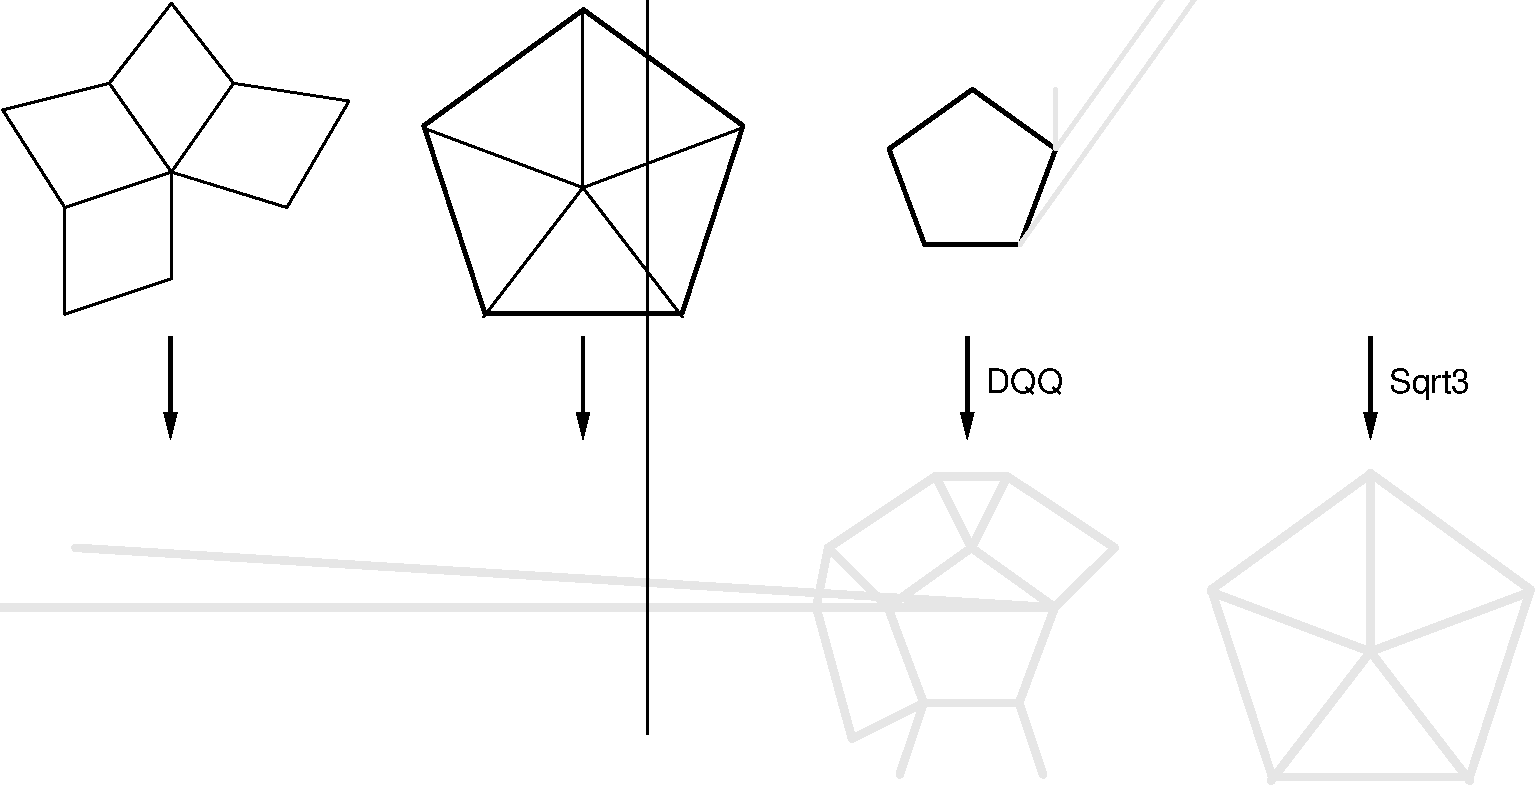
\includegraphics[width=0.6\textwidth]{\FIGDIR/RefSchemes}%
    }\\ \vspace{0.5cm}
    The refined mesh is shown below the control mesh.
  \end{center}
\end{ccTexOnly}

\begin{ccHtmlOnly}
  <CENTER>
     <img src="./FIG/RefSchemes.gif" alt="Refinement Hosts"></A><P>
  </CENTER>
\end{ccHtmlOnly}


\begin{ccExampleCode}
template <class Polyhedron>
class Subdivision_surfaces_3 {
  // S is the geometry policy realizing the geometry masks
  template <template <typename> class S>
  static void PQQ(Polyhedron& p, S<Polyhedron> rule, int step);

  template <template <typename> class S>
  static void PTQ(Polyhedron& p, S<Polyhedron> rule, int step);

  template <template <typename> class S>
  static void DQQ(Polyhedron& p, S<Polyhedron> rule, int step);

  template <template <typename> class S>
  static void Sqrt3(Polyhedron& p, S<Polyhedron> rule, int step);
}
\end{ccExampleCode}

%% Stencils are maintained using the iteration concept
%% to avoid the need for vertex tags to distinguish
%% the stencil types.
%% For example, on a PQQ refined mesh, the vertex iterator 
%% visits the 
%% vertex-nodes, edge-nodes and then facet-nodes. The visit
%% order is implicitly used to determine the stencil of
%% the visited node.

Each refinement host is a template function of
a mesh type and a policy type. The mesh type is
a model of the \ccc{CGAL::Polyhedron_3} concept, and the
policy type is a class with functions realizing the 
geometry masks of a specific subdivision scheme.
Refinement hosts refine the mesh, maintain the stencils 
(i.e.~the mapping between the control mesh and the refined mesh), 
and call policy functions to assign the smoothed points. 
The refinement is done by applying a sequence of connectivity 
operations (mostly are Euler operations).
The stencils are maintained by ordering new nodes to match the 
sequence of connectivity operations (which generate the refined nodes) 
of the refinement. By matching the ordering, no flag of the mesh
to indicate the stencils is required to maintain the stencils. 
Though to cooperate the geometry policies, \ccc{Point_3} type is 
required to be defined within the mesh. For details of the 
refinement algorithm and implementation, interested users should 
refer to \cite{cgal:sp-mrbee-05} .

% +-------------------------------------------------------------+
\section{Geometry Policy}
A geometry policy class defines a set of geometry masks. 
Each geometry mask is realized as a member function (i.e.~the policy) 
assigning new points according to the stencil weights.
%The policy interface is defined with the refinement host. 
Each policy function receives a primitive handle 
(e.g.~\ccc{Halfedge_handle}) of the control mesh, and the reference of 
the \ccc{Point} to the refined vertex. In general, the implementation of 
the policy function collects the neighbors of the primitive 
handle (i.e.~the stencil), and (ideally) computes the new point 
by a linear combination of the stencil 
points and the mask (i.e.~the stencil weights).
Following example shows an implementation of geometry masks 
of Catmull-Clark subdivision. \ccc{Point} is an alias to \ccc{Point_3}
in \ccc{Poly}.

\begin{ccExampleCode}
template <class Poly>
class CatmullClark_stencil_3 {
  //
  void facet_node(Facet_handle facet, Point& pt) {
    Halfedge_around_facet_circulator hcir = facet->facet_begin();
    int n = 0;
    FT p[] = {0,0,0};
    do {
      Point t = hcir->vertex()->point();
      p[0] += t[0], p[1] += t[1], p[2] += t[2]; 
      ++n;
    } while (++hcir != facet->facet_begin());
    pt = Point(p[0]/n, p[1]/n, p[2]/n);
  }
  //
  void edge_node(Halfedge_handle edge, Point& pt) {
    Point p1 = edge->vertex()->point();
    Point p2 = edge->opposite()->vertex()->point();
    Point f1, f2;
    facet_node(edge->facet(), f1);
    facet_node(edge->opposite()->facet(), f2);
    pt = Point((p1[0]+p2[0]+f1[0]+f2[0])/4,
               (p1[1]+p2[1]+f1[1]+f2[1])/4,
               (p1[2]+p2[2]+f1[2]+f2[2])/4 );
  }
  //
  void vertex_node(Vertex_handle vertex, Point& pt) {
    Halfedge_around_vertex_circulator vcir = vertex->vertex_begin();
    int n = circulator_size(vcir);    

    float Q[] = {0.0, 0.0, 0.0}, R[] = {0.0, 0.0, 0.0};
    Point& S = vertex->point();
    
    Point q;
    for (int i = 0; i < n; i++, ++vcir) {
      Point& p2 = vcir->opposite()->vertex()->point();
      R[0] += (S[0]+p2[0])/2;
      R[1] += (S[1]+p2[1])/2;
      R[2] += (S[2]+p2[2])/2;
      facet_node(vcir->facet(), q);
      Q[0] += q[0];      
      Q[1] += q[1];      
      Q[2] += q[2];
    }
    R[0] /= n;    R[1] /= n;    R[2] /= n;
    Q[0] /= n;    Q[1] /= n;    Q[2] /= n;
      
    pt = Point((Q[0] + 2*R[0] + S[0]*(n-3))/n,
               (Q[1] + 2*R[1] + S[1]*(n-3))/n,
               (Q[2] + 2*R[2] + S[2]*(n-3))/n );
  }
}
\end{ccExampleCode}

The interfaces of a geometry policy need to match the stencils of 
the refinement host. A PQQ refinement host requires three 
policy functions for meshes without open boundaries: a vertex-node 
stencil, an edge-node stencil, and a facet-node stencil. 
To support meshes with boundaries, a policy function
for border vertices is also required.

%% \begin{ccTexOnly}
%%   \begin{center}
%%     \parbox{0.5\textwidth}{%
%%       
\includegraphics[width=0.5\textwidth]{\FIGDIR/PQQStencil}%
%%     }
%%   \end{center}
%% \end{ccTexOnly}

%\begin{ccHtmlOnly}
%  <CENTER>
%  <A HREF="./FIG/PQQStencil.gif">
%     <img src="./FIG/PQQStencil.gif" alt="Stencils of PQQ scheme "></A><P>
%  </CENTER>
%\end{ccHtmlOnly}


\begin{ccExampleCode}
  void border_node(Halfedge_handle edge, Point& ept, Point& vpt) {
    Point& ep1 = edge->vertex()->point();
    Point& ep2 = edge->opposite()->vertex()->point();
    ept = Point((ep1[0]+ep2[0])/2, (ep1[1]+ep2[1])/2, (ep1[2]+ep2[2])/2);

    Halfedge_around_vertex_circulator vcir = edge->vertex_begin();
    Point& vp1  = vcir->opposite()->vertex()->point();
    Point& vp0  = vcir->vertex()->point();
    Point& vp_1 = (--vcir)->opposite()->vertex()->point();
    vpt = Point((vp_1[0] + 6*vp0[0] + vp1[0])/8,
                (vp_1[1] + 6*vp0[1] + vp1[1])/8,
                (vp_1[2] + 6*vp0[2] + vp1[2])/8 );
  }
\end{ccExampleCode}


The interface of PQQ, PTQ, DQQ and $\sqrt{3}$ refinement hosts are 
defined below:


\begin{ccExampleCode}
template <class Poly>
class PQQ_stencil_3 {
  void facet_node(Facet_handle, Point&) {};
  void edge_node(Halfedge_handle, Point&) {};
  void vertex_node(Vertex_handle, Point&) {};

  void border_node(Halfedge_handle, Point&, Point&) {};
};

template <class Poly>
class PTQ_stencil_3 {
  void edge_node(Halfedge_handle, Point&) {};
  void vertex_node(Vertex_handle, Point&) {};

  void border_node(Halfedge_handle, Point&, Point&) {};
};

template <class Poly>
class DQQ_stencil_3 {
public:
  void corner_node(Halfedge_handle edge, Point& pt) {};
};

template <class Poly>
class Sqrt3_stencil_3 {
public:
  void vertex_node(Vertex_handle vertex, Point& pt) {}
};
\end{ccExampleCode}

Note in current implementation, \ccc{DQQ_stencil_3} and 
\ccc{Sqrt3_stencil_3} do not support
meshes with global boundaries; though these might be changed
in the future release. Also, \ccc{PTQ_stencil_3} and
\ccc{Sqrt3_stencil_3} are subset of \ccc{PQQ_stencil_3}, and are not
explicitly defined in \ccc{Subdivision_surfaces_3}.

%% \begin{ccExampleCode}
%% PQQ<_M,CCstencil>(Mesh,CCstencil<_M>())
%% \end{ccExampleCode}
%% (or, more simply \\
%% \begin{ccExampleCode}
%% PQQ(Mesh,CCstencil<_M>())}
%% \end{ccExampleCode}
%% since the compiler can derive the template
%% arguments from the function parameters),
%% instantiates Catmull-Clark subdivision.    
%% \ccc{_M}, the model of the mesh concept,
%% represents the mesh type (\ccc{Mesh}),
%% and \ccc{CCstencil} is a class template 
%% realizing geometry policies of Catmull-Clark subdivision.

%The geometry stencils of Catmull-Clark subdivision (border stencils are 
%not included) are shown below. 

%\begin{ccTexOnly}
%  \begin{center}
%    \parbox{0.4\textwidth}{%
%      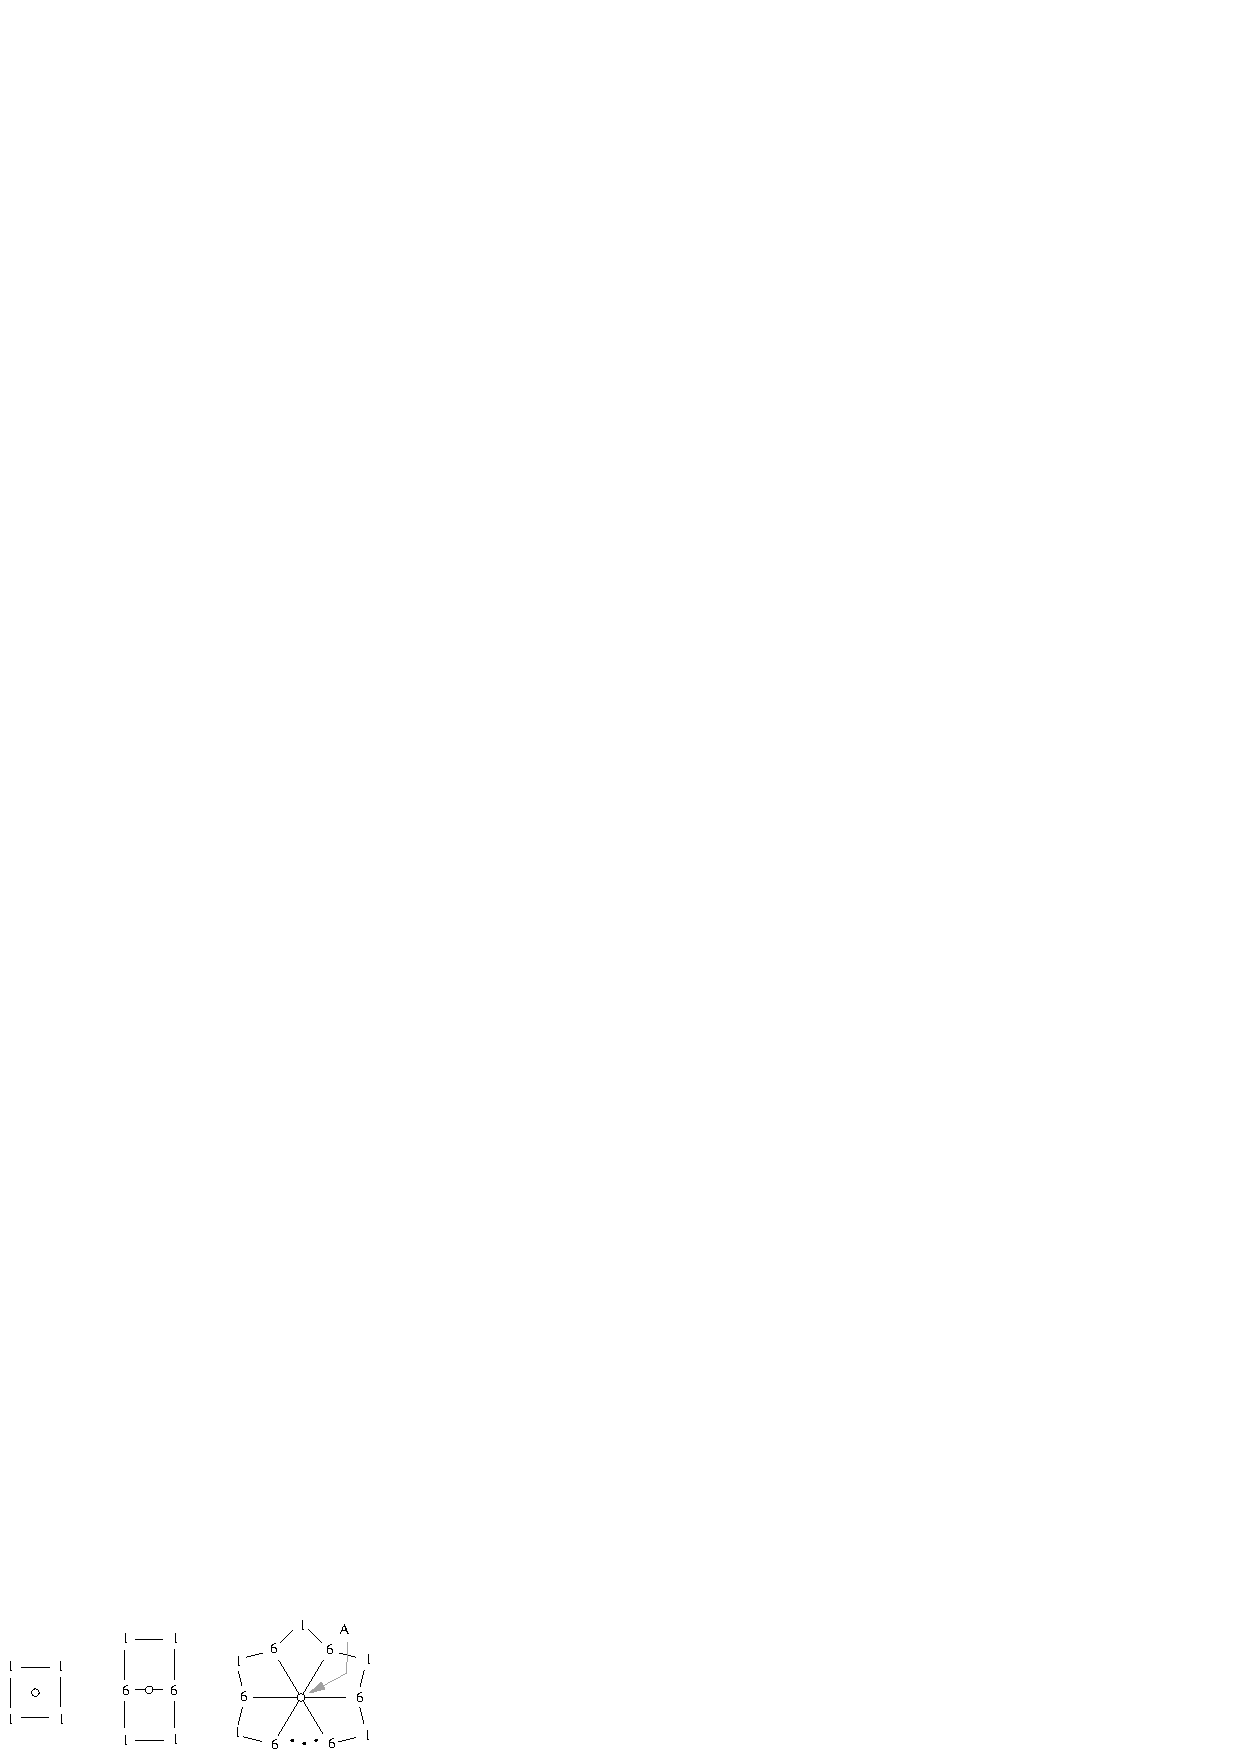
\includegraphics[width=0.4\textwidth]{\FIGDIR/cc_mask}%
%    }
%  \end{center}
%\end{ccTexOnly}

%\begin{ccHtmlOnly}
%  <CENTER>
%  <A HREF="./FIG/cc_mask.gif">
%     <img src="./FIG/cc_mask.gif" alt="Catmull-Clark geometry stencil"></A><P>
%  </CENTER>
%\end{ccHtmlOnly}


% +------------------------------------------------------------------------+
\section{Built-in subdivision schemes}
% +------------------------------------------------------------------------+
Considering their popularity in graphics modeling, 
Catmull-Clark, Loop, \DS\ and $\sqrt{3}$ subdivisions are directly
supported in \ccc{Subdivision_surfaces_3}. 
%Each of these subdivision schemes is realized by parameterizing 
%the corresponding geometry policy to the .

\begin{ccExampleCode}
  static void CatmullClark_subdivision(Polyhedron& p, int step) {
    PQQ(p, CatmullClark_stencil_3<Polyhedron>(), step);
  }
  static void Loop_subdivision(Polyhedron& p, int step) {
    PTQ(p, Loop_stencil_3<Polyhedron>() , step);
  }
  static void DooSabin_subdivision(Polyhedron& p, int step) {
    DQQ(p, DooSabin_stencil_3<Polyhedron>(), step);
  }
  static void Sqrt3_subdivision(Polyhedron& p, int step) {
    Sqrt3(p, Sqrt3_stencil_3<Polyhedron>(), step);
  }
\end{ccExampleCode}

Following shows an example of \DS\ subdivision on a polyhedral mesh.
\ccIncludeExampleCode{Subdivision_surfaces_3/DooSabin_subdivision.C}

% +------------------------------------------------------------------------+
\section{Customize subdivision schemes}
% +------------------------------------------------------------------------+
The goal of \ccc{Subdivision_surfaces_3} is to provide a flexible platform
to develop user-flavored subdivision schemes.
To construct a customized subdivision scheme, users can simply 
choose a refinement host with the intended topological pattern, 
and then realize the geometry policy accordingly. 
Following example develops a subdivision scheme
generating improved Loop subdivision surfaces based on the PTQ 
refinement (i.e~\ccc{Subdivision_surfaces_3<Polyhedron>::PTQ}). 
The geometry policy is developed as a subclass 
of \ccc{PQQ_stencil_3}, which defines the superset of PTQ stencils.

A policy function for subdivision surfaces is semantically
required to assigned the smoothed point based on the source mesh.

\ccIncludeExampleCode{Subdivision_surfaces_3/Customized_subdivision.C}
